\begin{figure}[htb]
	\centering
	\begin{subfigure}{0.45\linewidth}
		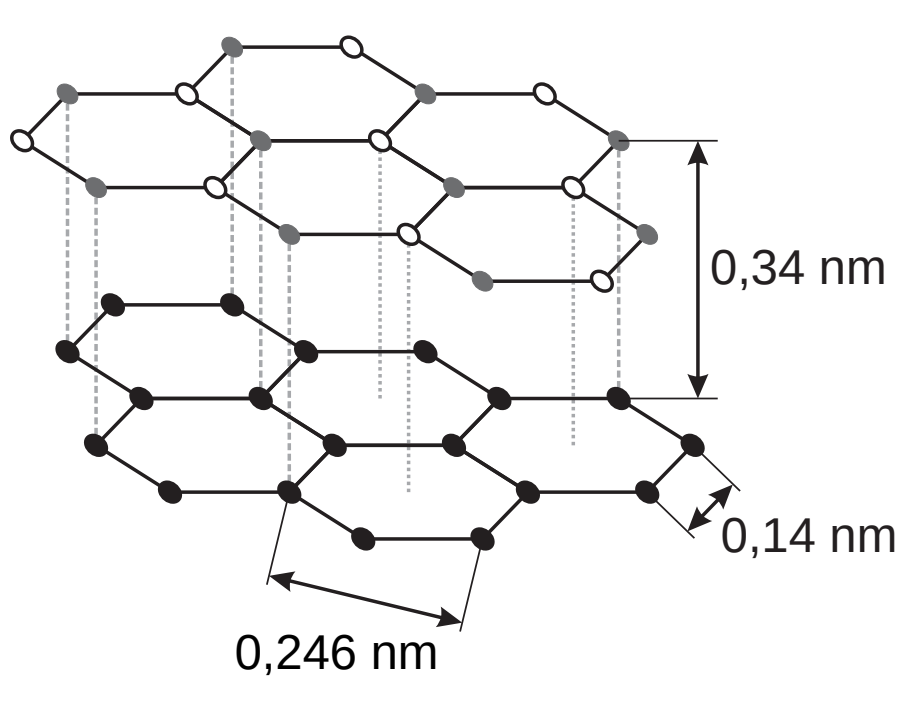
\includegraphics[width=\linewidth]{figs/hopg1.png}
		\caption{Seitenansicht.\cite[S.49]{skript}}
		\label{fig:hopg1}
	\end{subfigure}
	\hspace{0.5cm}
	\begin{subfigure}{0.45\linewidth}
		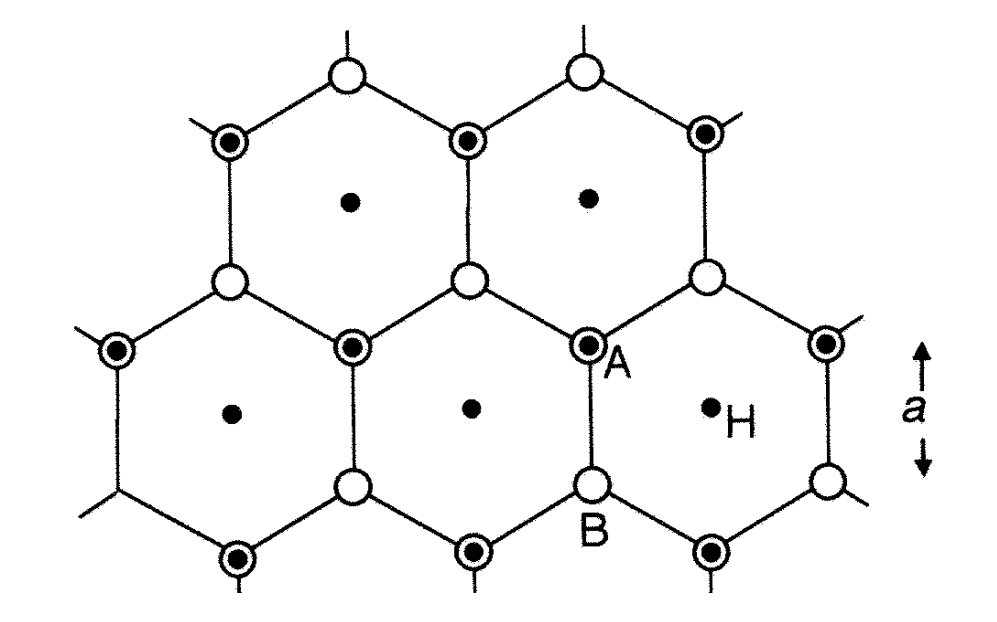
\includegraphics[width=\linewidth]{figs/hopg2.png}
		\caption{Obere Ansicht.\cite[Kap.1 S.17]{rtm-leitpfaden}}
		\label{fig:hopg2}
	\end{subfigure}
	\caption{Hochorientierter pyrolyitscher Graphit.}
	\label{fig:hopg-skizze}
\end{figure}